 \documentclass[]{article}
\usepackage{graphicx}
\usepackage{cite}
\usepackage{subfigure}
\usepackage{amsmath}
\usepackage{amssymb}
%\usepackage{doublespace}
% \usepackage{fullpage}
\usepackage{fancyhdr}
\usepackage{url}
\usepackage{algorithm}
\usepackage{algorithmic}
\usepackage{xspace}
\usepackage{amsthm}
\usepackage{enumitem}


\usepackage{color}
\newcommand{\hilight}[1]{\colorbox{yellow}{#1}}
\usepackage{layouts}  %helps print textheight and textwidth in inches...it's about 8.5 but I'm only getting 6 in height inside a figure environment
\usepackage{multirow}
\usepackage{rotating}  % To put figures with their captions sideways
\usepackage[top=2.0in, bottom=1.5in, left=1in, right=1in]{geometry}
\usepackage[section]{placeins}

%%EXAMPLES: 
%\begin{sidewaysfigure}%\begin{center}
%\includegraphics[width=1.0\textwidth]{figs/Our-territory.pdf}
%\caption{We show the activities of the project in Year 1 in the context of evolutionary systems.}
%\label{fig:our-activities}%\end{center}%\end{sidewaysfigure}
%
%\begin{sideways}
%Is this rotated?  YES! IT IS!!
%\end{sideways}
%

%\usepackage{hyperref}  % see below for colouring options included
\usepackage[bookmarks=false,colorlinks=true,linkcolor={blue},citecolor={blue},urlcolor={blue}]{hyperref}

%
%
%

% additional packages included in Daniele's thesis:
\usepackage[italian,english]{babel} %to set the language
\usepackage{tabularx} %to use tabular environment
\usepackage{amsmath} %to manage math formulas
\usepackage{amssymb} %to manage math formulas
%\usepackage[scriptsize]{caption} %to customise the captions
\usepackage{stdclsdv} %to control the design of the contents
%\usepackage{tocloft} %to control the design of the contents
\usepackage[usenames,dvipsnames,svgnames,table]{xcolor} %to manage the colors
\usepackage{fancyhdr} %to use the fancy style
\usepackage{caption} %to manage rotated subfigures
\usepackage{wrapfig}
\usepackage{listings}
\usepackage{pgf}



%\makenomenclature
%\setcounter{secnumdepth}{3}
%\setcounter{tocdepth}{3}

\def \nibf#1{\noindent\textbf{#1}}
%\newcommand{\NB}[1]{\textcolor{red}{\textbf{Comment: #1}}}
%\newcommand{\UM}[1]{\textcolor{blue}{\textbf{UM: #1}}}

%\newcommand{\TODO}[1]{\textcolor{red}{\textbf{TODO: #1}}}
%\newcommand{\CHECK}[1]{\textcolor{red}{\textbf{CHECK THIS: #1}}}
%\newcommand{\RedBF}[1]{\textcolor{red}{\textbf{#1}}}
%\newcommand{\BlueBF}[1]{\textcolor{blue}{\textbf{#1}}}
%\newcommand{\redbf}{\RedBF}
%\newcommand{\bluebf}{\BlueBF}

\usepackage{tocloft}
\newcommand{\listappendicesname}{Appendices}
\newlistof{appendices}{apc}{\listappendicesname}
\newcommand{\appendices}[1]{\addcontentsline{apc}{appendices}{#1}}

\newcommand{\newappendix}[1]{\section*{#1}\appendices{#1}}
%set the abbreviations



%-------------------------------------------------------------------------
\begin{document}
\begin{titlepage}
\begin{center}


{ \Large\bfseries CommunityFinder: Software to Analyze Communities that Develop in MOOC Discussion Forums}\\

\vspace{2cm}
 
{\large \bf Max Kanter}
{\large \bf Kalyan Veeramachaneni}



 \textsc{Any Scale Learning for All}\\
 Computer Science and Artificial Intelligence Laboratory\\
 Massachusetts Institute of Technology

\end{center}
\end{titlepage}



\tableofcontents
\newpage
\listoffigures
\newpage
\listoftables
\newpage
\listofappendices
\newpage

\pagestyle{plain}
\lfoot{\today}
\cfoot{\thepage}
\rfoot{ALFA, CSAIL, MIT}
\pagestyle{plain}
\pagenumbering{arabic}
\setcounter{page}{1}
\newpage
\section*{Abstract}

CommunityFinder is software to analyze the communities that develop in massively online open courses (MOOCs).  The goal of the tool is to give researchers and teachers further insight into their classes. The software organizes a corpus of forum posts into an Interaction Graph that represents how students interact with each other. From this graph, the software can perform community detection using two different algorithms. Along with the source code, we also release the results of running CommunityFinder on two different edX courses.

\section{Introduction}
Massively online open courses, or MOOCs, are offered by universities across the country, including MIT. Over 100 classes are offered on platforms like edX and Coursera and this number is growing. Due to the nature of being online and open, a lot of data is being collected about how students interact with the course material.

The discussion forums in these classes are the primary way that students and teachers interact in these online courses. For example, the first offering of 6.002x  (Circuits and Electronics) in Spring 2012 had over 90,000 posts made.

In this paper, we present CommunityFinder, which is software that extracts structured representation of how student interact with MOOCs and then performs community analysis on this structured representation. The software outputs information on several aspects of the community structure in an online course.


\section{Motivation} 
Understanding the community structure of a graph can bring improved understanding of complex systems. MOOCs provide a new complexity to education in not only the size of their enrollment, but also in the different way that they teach material. If we understand qualitatively how students interact with each other and instructors in a course, we will be able to better understand how successes and failures of MOOCs. This understanding will allow educators to improve these online course moving forward.

\section{Previous Work}
The problem of identifying communities is very hard and not yet satisfactorily solved. The dependency on domain makes it difficult to generate general purpose algorithms. Further, some domains such as social network data require not only accurate, but efficient algorithms to process large amounts of data. However, there is a large interdisciplinary effort to solve it because of the number of applications.

The community structure in a network of interactions represented as a graph where entities are vertices and interactions are edges is a clustering of a graph such that vertices in a cluster have more edges to vertices in the same cluster and fewer edges to vertices in other clusters\cite{2010PhR...486...75F}. How we interpret the clusters that form is often dependent on the domain of the problem, but they often are interpreted as vertices playing a similar role. For example, given an network of how scientific researchers have collaborated with each other, we would expect to find that communities correspond to the different scientific disciplines. 

In the domain of online education, we might want to identify the students that take various roles in a class. Huang et al. \cite{Huang:2014:SBM:2556325.2566249} focused on the most focal subset of contributors on MOOC forum that they label as \emph{superposters}. They suggest the \emph{superposters} can be models for the ideal student because they often make high quality posts. Their study seeks to examines contribution patterns, demographics, and course performance and enrollment of these \emph{superposters}. The researchers conclude that these posters make high-value contributions and also encourage further student engagement. 

Other researchers analyzed post content from business strategy class on Coursera \cite{DBLP:journals/corr/GillaniEOHR14}. This meant considering over 15,600 posts. They looked at 5 aspects a student's postings and then used Bayesian Non-negative Matrix Factorization to extract communities. They looked specifically at two sub-forums and identified communities such as committed crowd engagers, discussion initiators, strategists, and individuals.


\section{Student Relationships in Discussion Forums}

\begin{wrapfigure}{r}{0.6\linewidth}
  \begin{center}
    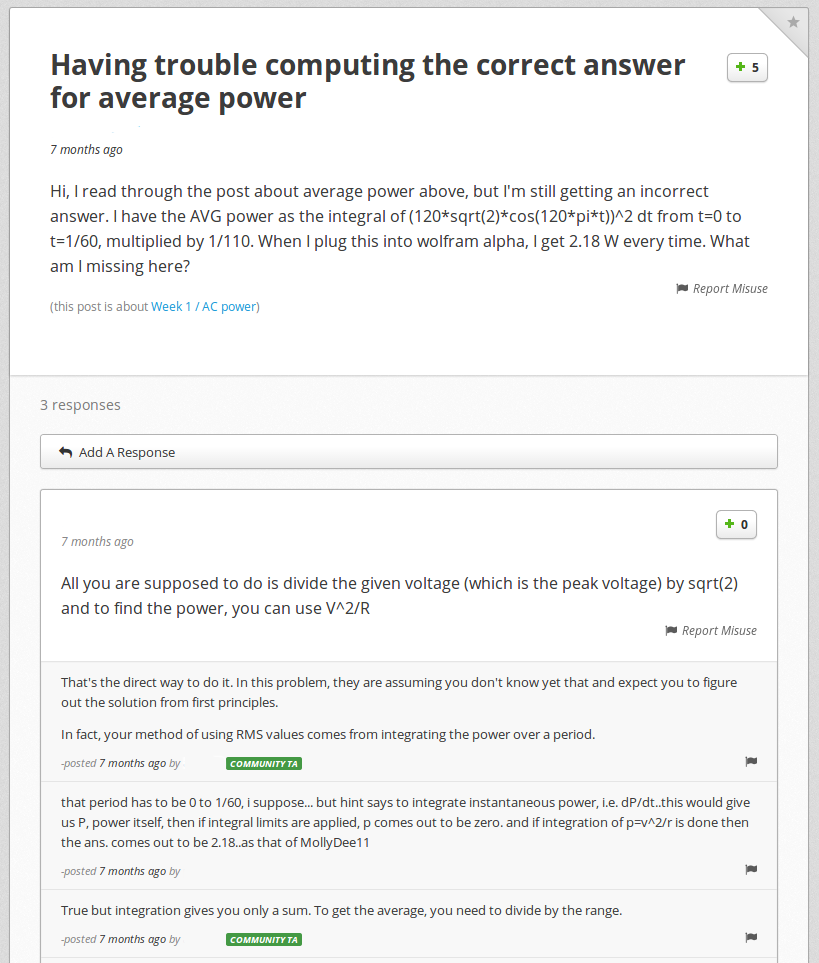
\includegraphics[width=1\linewidth]{forum_example.png}
    \caption{An example thread from 6.002x Spring 2014, which is currently being offered.}
    \label{forum}
  \end{center}
\end{wrapfigure}

Students interact in the discussion forums. Because of this, we can infer inter-student relationships based on a corpus of forum posts. 

The discussion forms we consider in this paper are organized as a collections of threads. Within a thread, students have the opportunity to converse with each other on a common topic. Figure \ref{forum} is an example thread from a class currently being offered on edX.

We rely on the thread structure of the conversations to determine student relationships. A thread is a hierarchy of posts where every post besides the first has a parent post that it is associated with. The parent/child relationship is interpreted as the child post being a reply to the parent. We use this interpretation to say author of a child post has interacted with the author the parent post. We only consider the immediate parent. 

We consider two students to be related if they interact in a thread. The strength of this relationship is determined by how often one student replies to another. The idea is that the more often we find one student replying to another, the more likely are in the same communitiy.

Using this understanding of how students who post on the forum are related, we present the idea of an Interaction Graph. 

\subsection{Interaction Graph}
\begin{figure}[h]
  \centering
  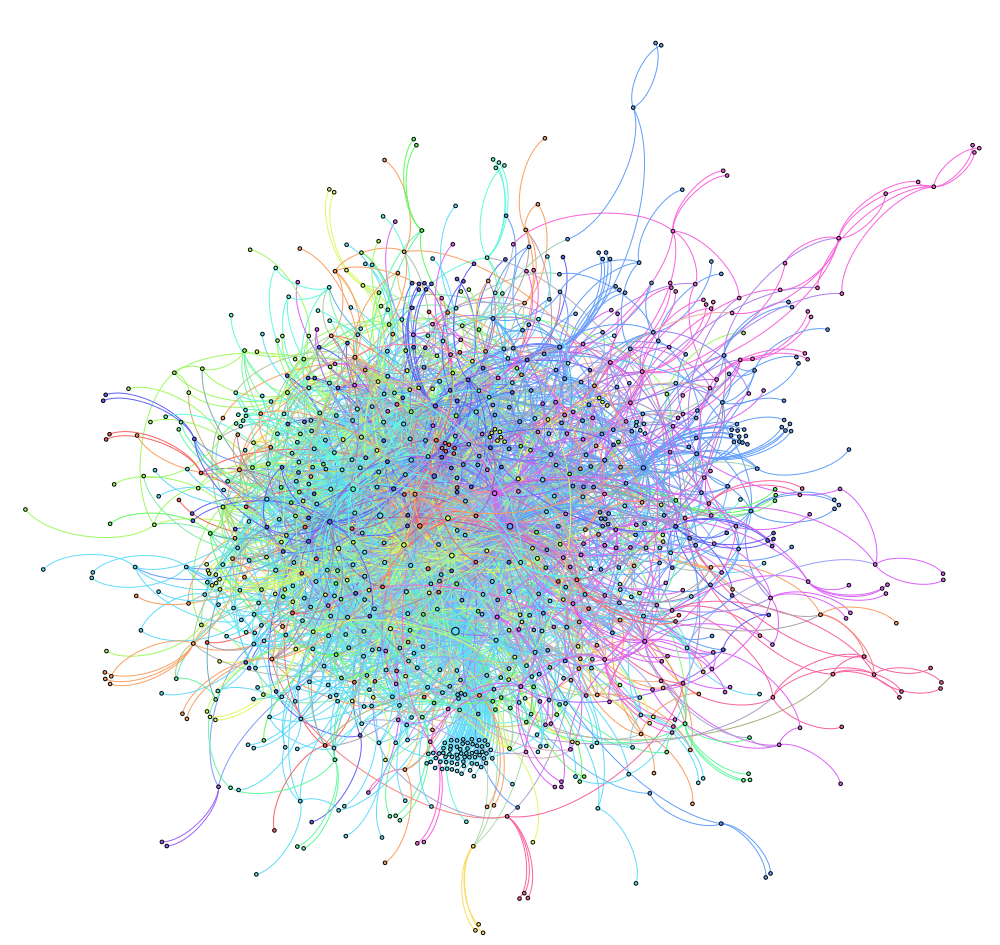
\includegraphics[width=.7\linewidth]{interaction_graph.png}
  \caption{This is a visualization of the Interaction Graph for 6.002x Fall 2012. This graph has 2163 students who made 6902 posts.}
  \label{interactions}
\end{figure}

In an Interaction Graph, each vertex represents a student in the class. For two students $i$ and $j$, the graph has a directed edge from $i$ to $j$ if $i$ has made a comment in direct reply to $j$. The edge between $i$ and $j$ is weighted by the number of times that $i$ directly replied to $j$ across all threads in the forum. We use this directed and weighted model to preserve as much information as possible about the the original forum interactions. Only students who are involved in a thread with at least one reply are considered. Figure \ref{interactions} shows what the graph of student interactions looks like for 6.002x offered in Fall 2012.

\section{Community Detection}
We considered two different approaches to identifying communities: spectral clustering and Louvain Method.
\begin{figure}[!htb]
  \centering
  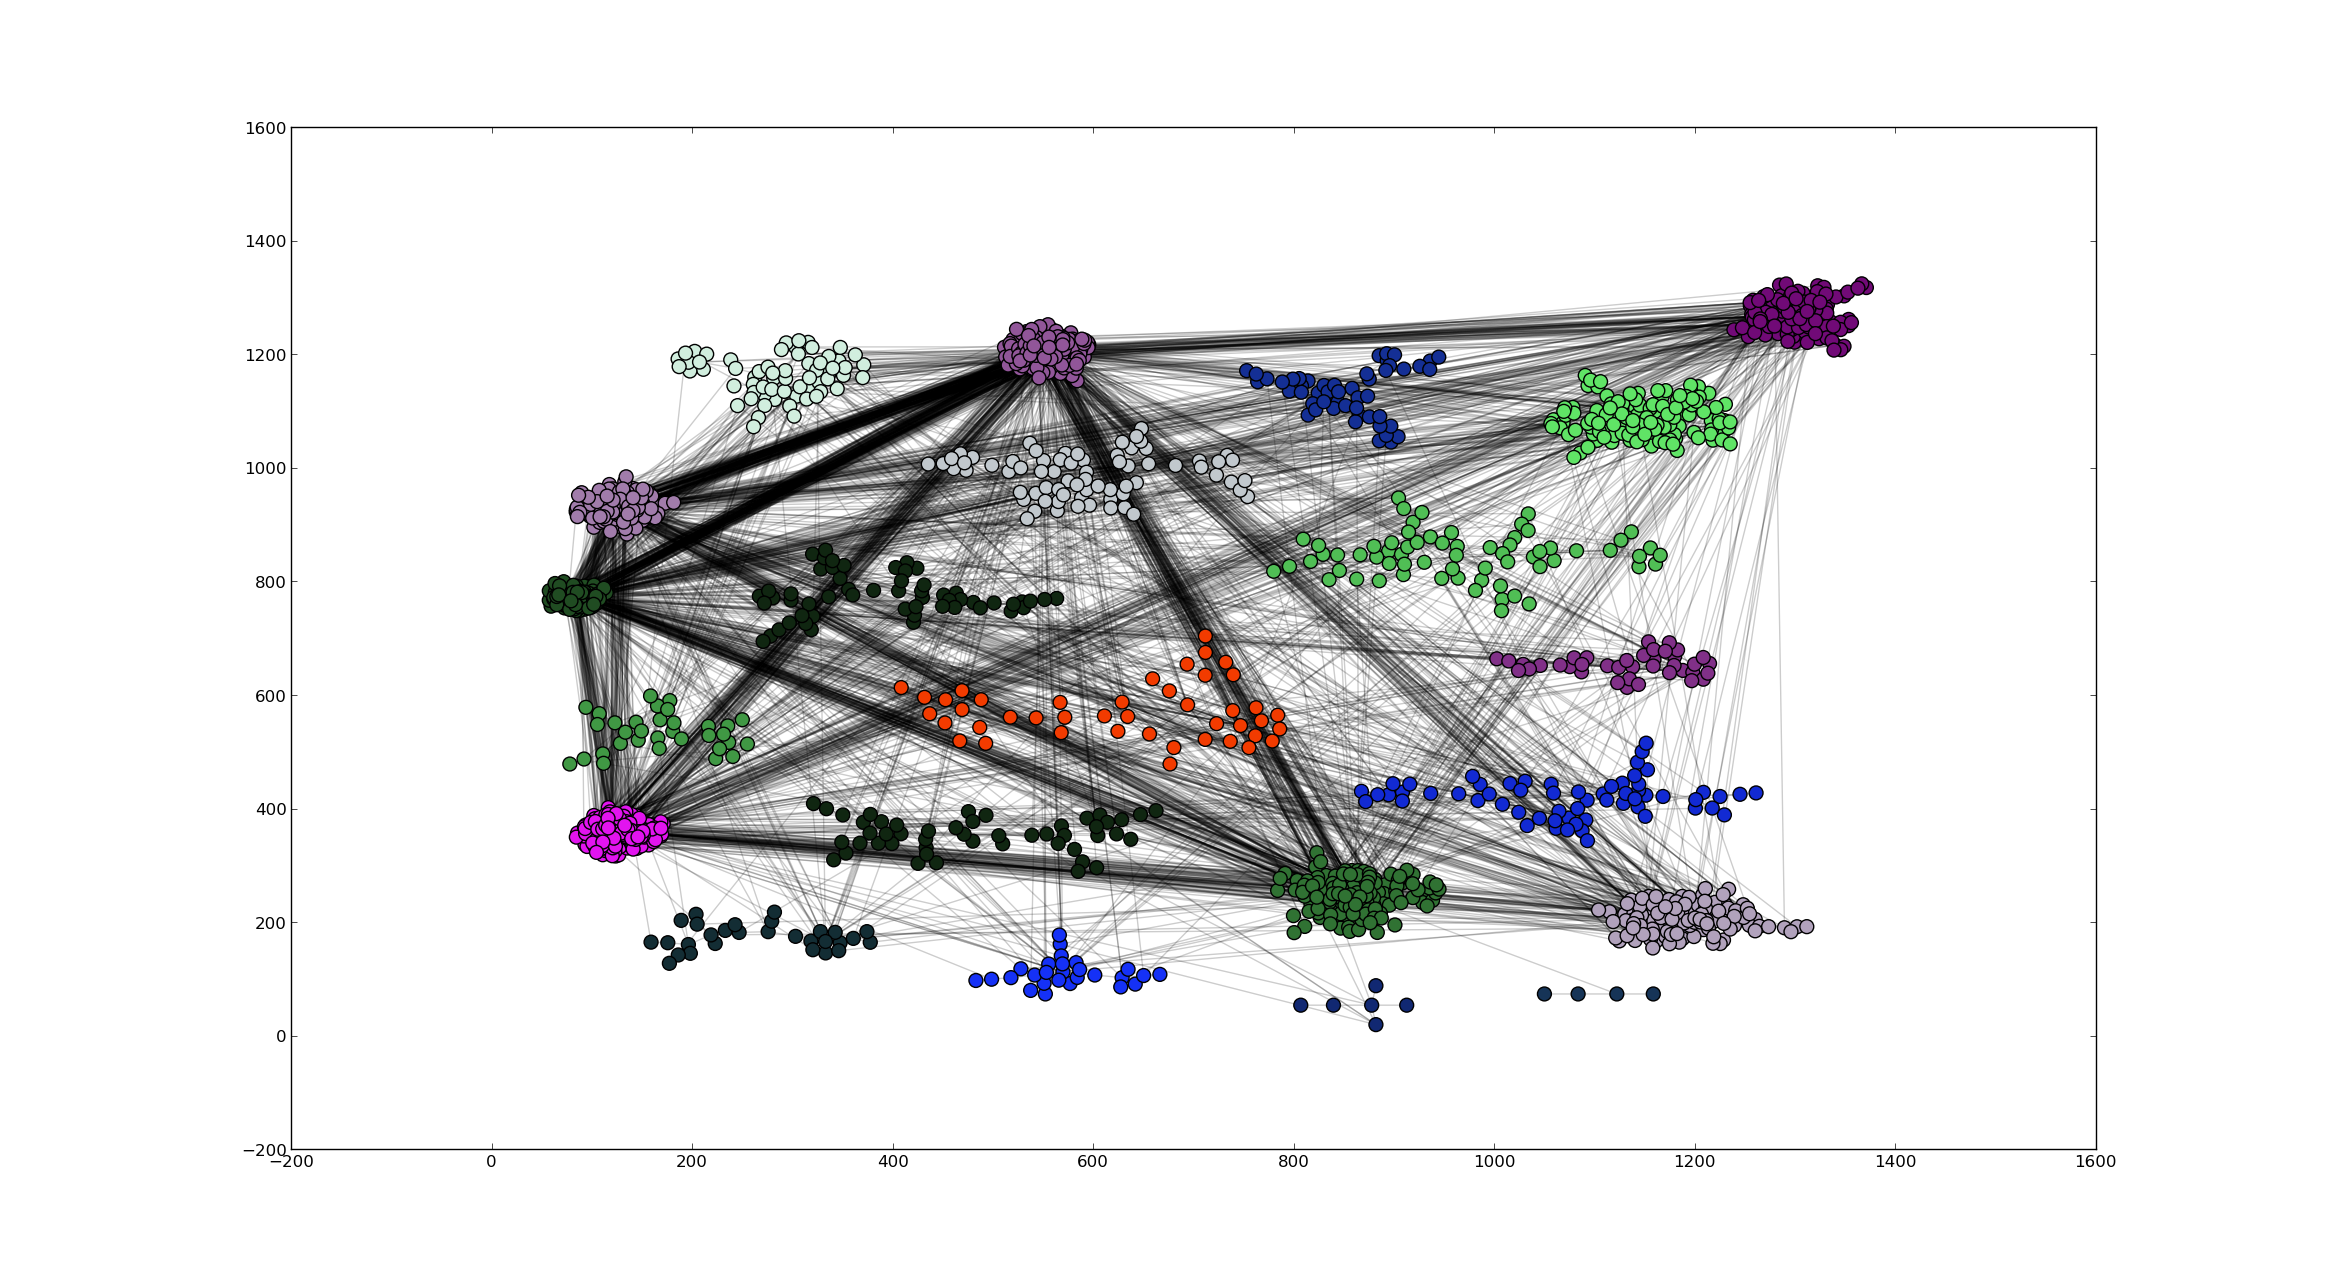
\includegraphics[width=.8\linewidth]{louvain_best.png}
  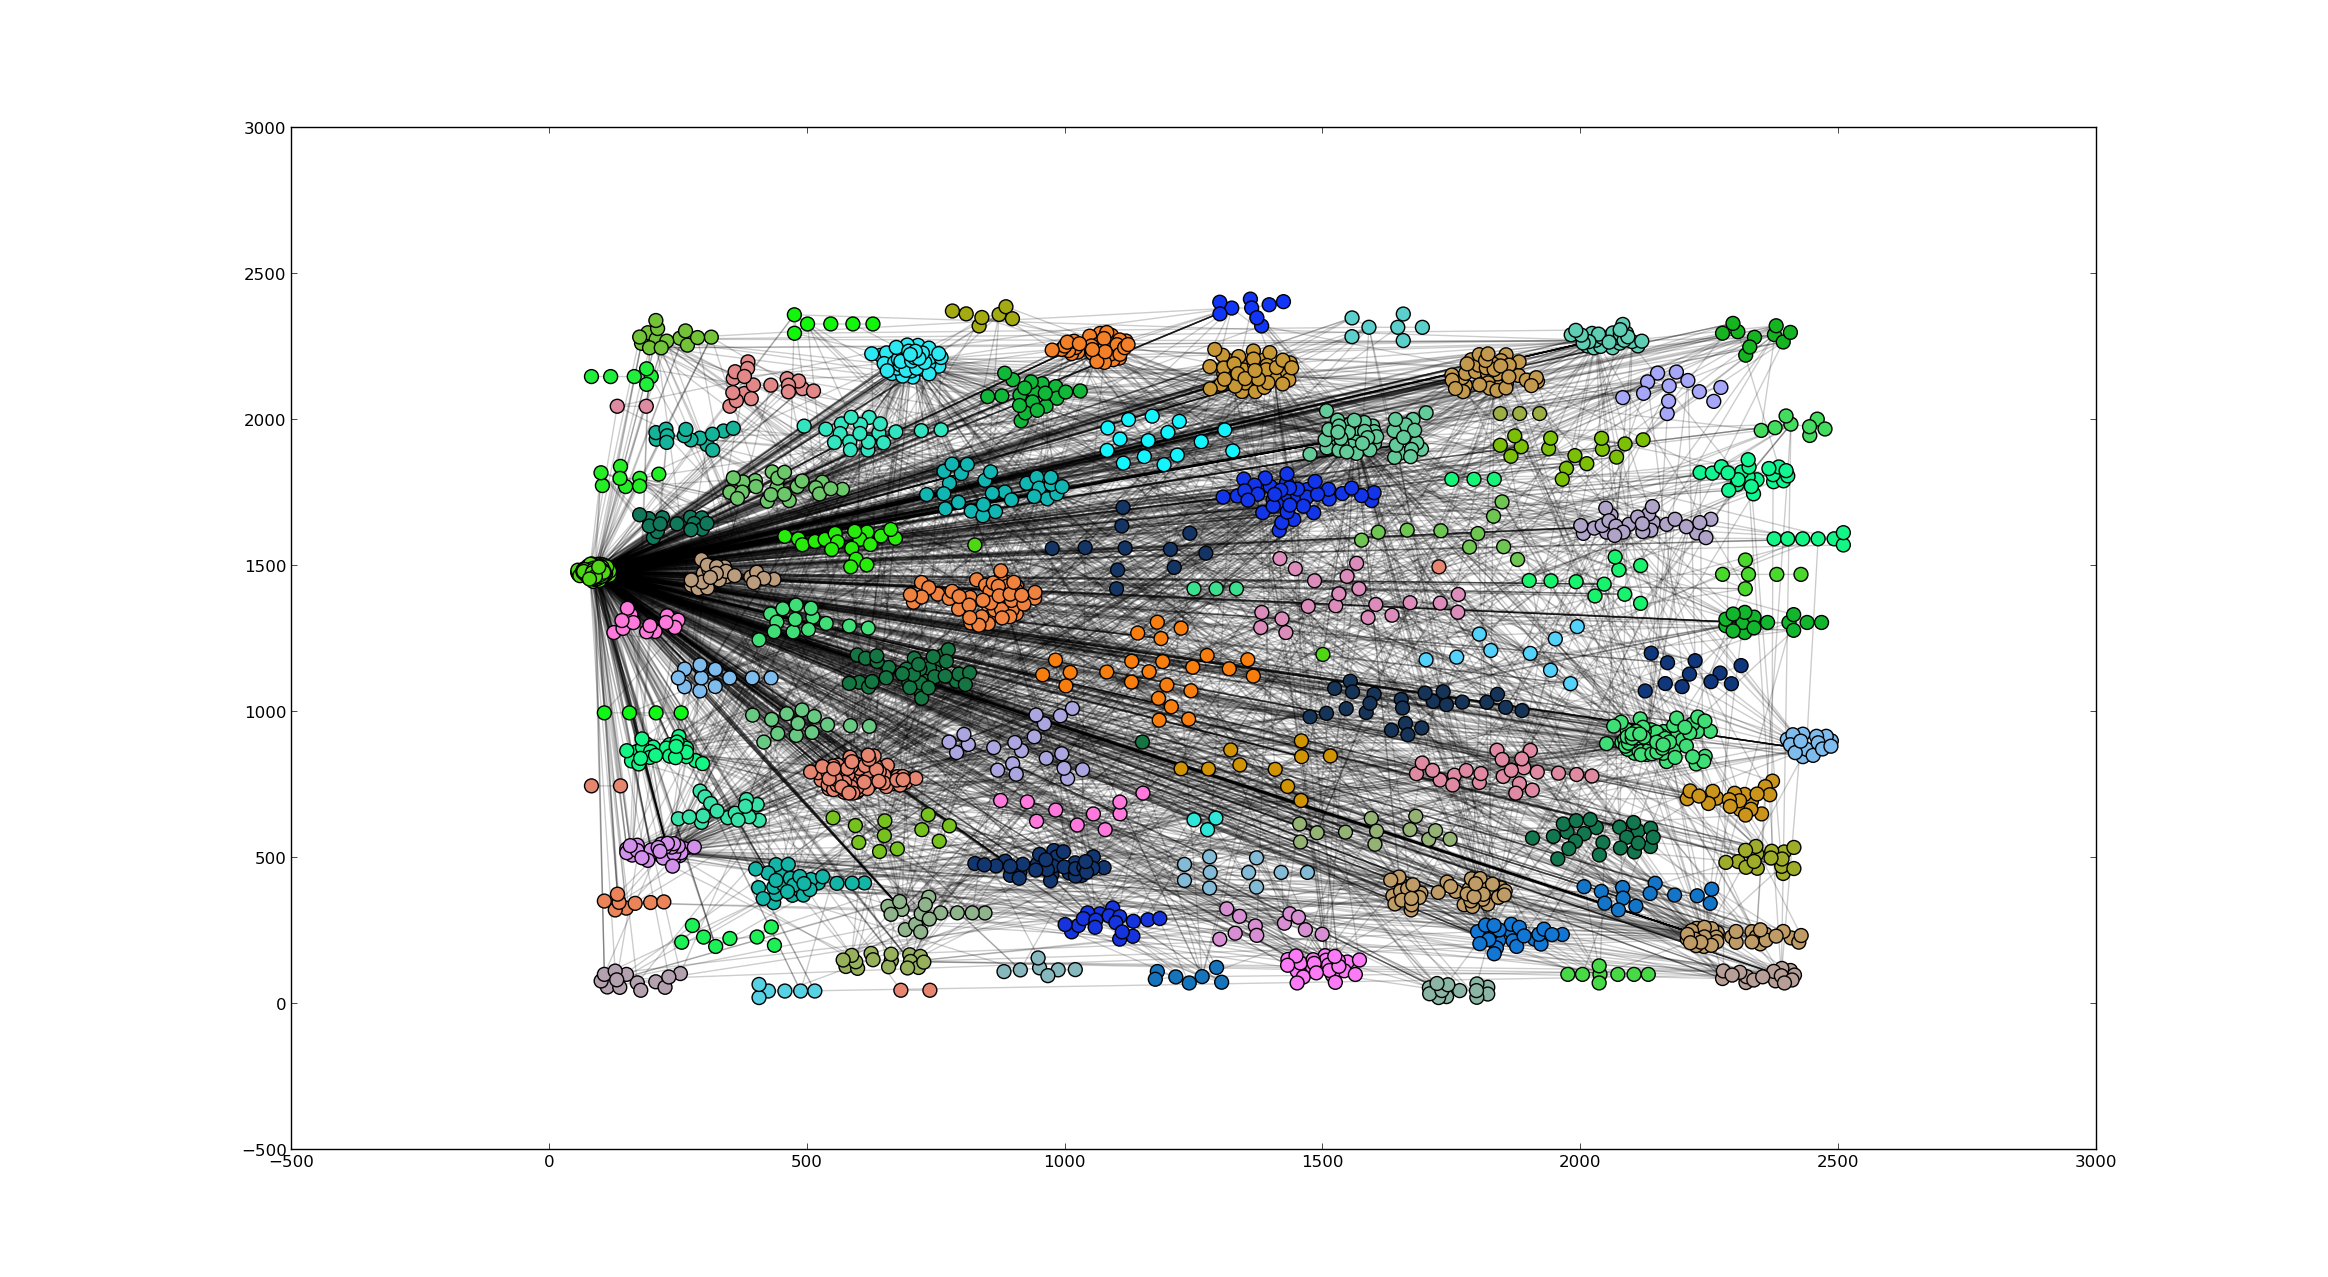
\includegraphics[width=.8\linewidth]{spectral_best.png}
  \caption{Visualization of the results of the highest modularity partitioning of 6.002x Fall 2012. On the top is the the best Louvain Method partition. On the bottom is the best spectral clustering partition.}
  \label{Louvain_best}
\end{figure}

\subsection{Spectral Clustering}

Spectral clustering is a group of techniques that transforms the initial set of verticies in space by using eigenvectors. After this transformation, the points are clustered using a standard algorithm\cite{2010PhR...486...75F}. Spectral clustering can be broken down into 3 parts

\begin{description}
  \item[Affinity Matrix] The algorithm uses an affinity matrix that describes the similarity between two vertices. In our case, the affinity matrix is exactly an instance of the Interaction Graph. This works because the $ij$ entry of an Interaction Graph encodes how the strength of the relationship between $i$ and $j$. 
  
  \item[Dimension Reduction] The algorithm uses the spectrum of the graph Laplacian to reduce the dimension of the matrix.  The Laplacian, L, of the graph is defined as 
  \begin{equation}
  L = D - A
  \end{equation}
  where $D$ is a diagonal matrix with $d_{ii} = deg[i]$ and $A$ is the adjacency matrix. In our implementation\footnote{In this paper, we use an implementation of spectral clustering and discrete clustering provided by scikit-learn\cite{spectral}.}, we use the normalized graph Laplacian which is defined as 
  \begin{equation}
  L' = D^{-\frac{1}{2}}LD^{-\frac{1}{2}}
  \end{equation}
  
  This is preferred to the unnormalized Laplacian because it performs better under general conditions \cite{von2008consistency}. Using the eigenvectors of the normalized Laplacian, each vertex is transformed into a lower dimension space where the coordinates are elements of the eigenvectors. This reduction is important because it makes the important features of the initial matrix more prominent before applying clustering. Thus, this method allows clusters to be identified that would not have been identified by standard clustering techniques. For example, spectral clustering tends to transform the initial into points into a convex sets of points, which are easier to cluster\cite{2010PhR...486...75F}.
  
  \item[Clustering] The algorithm uses a discrete method proposed by Yu and Shi to do clustering in the lower dimension space. This method was chosen over KMeans for clustering because it is often faster and more robust to random initialization than KMeans\cite{yu2003multiclass}. The clustering is found by iteratively searching for a discrete partition closest to the eigenvector embedding. This done by first normalizing the eigenvector embedding to the space of the partition matrix. Next, a we fix an optimal discrete partition matrix and then calculate the optimal rotation matrix. These to steps are performed until convergence. The discrete partition matrix is returned as the solution to the clustering problem. 
 
\end{description}

\subsection{Louvain Method}
The Louvain method is a greedy optimization method for determining communities in large networks \cite{2008JSMTE..10..008B}. It seeks to optimize the modularity of a partition of the network. Given a partition of the graph, the modularity measures the relative frequency of links inside communities as compared to links between communities. It is scalar value between -1 and 1 and is calculated as follows

\begin{equation}
Q = \frac{1}{2m} \sum_{i,k} \left[ A_{ij} - \frac{k_i k_j}{2m}\right]\delta(c_i,c_j)
\end{equation}

where $A_{ij}$ is the weight of the edge between $i$ and $j$, $k_i = \sum_{j}A_{ij}$, $c_i$ is the community that $i$ is assigned to, the $\delta(u,v)$ is 1 if $u=v$ and 0 otherwise, and $m = \frac{1}{2}\sum_{ij}A_{ij}$. 

Exact modularity optimization is NP-hard \cite{2008JSMTE..10..008B}. The algorithm starts by assigning a unique community to each node and then iteratively performing two steps until maximum modularity is achieved. First, the method looks at every node $i$ and its each of its neighbors $j$. Node $i$ is removed from its community and added to the community of $j$ where the gain in modularity is highest. If the modularity cannot be improved by moving $i$, then the community assignment will not change. This is repeated until no more changes in community can be performed to increase modularity. The second step is to build a new network where the nodes are the communities discovered in the first step. Edges between nodes in the same community are self loops in the is new graph. These steps are repeated iteratively until no more changes occur during an iteration, which means a maximum of modularity has been reached. This produces a hierarchy of communities. This method has been observed to be very fast and appears to run in $O(nlogn)$\cite{2008JSMTE..10..008B}, where $n$ is the number of nodes in the network\footnote{In this paper, we use an implementation for directed graphs for the NetworkX library \cite{louvain}.}.





\section{CommunityFinder Software}

\subsection{Overview}
CommunityFinder identifies the community structure in a set of forum posts. It does this by infering the strength of a pair of students' relationship based on how often they make posts to each other. After this structure is determined for all students, CommunityFinder offers two methods of inferring the community structure implied by student interactions. 

\begin{figure}[h]
 \centering
 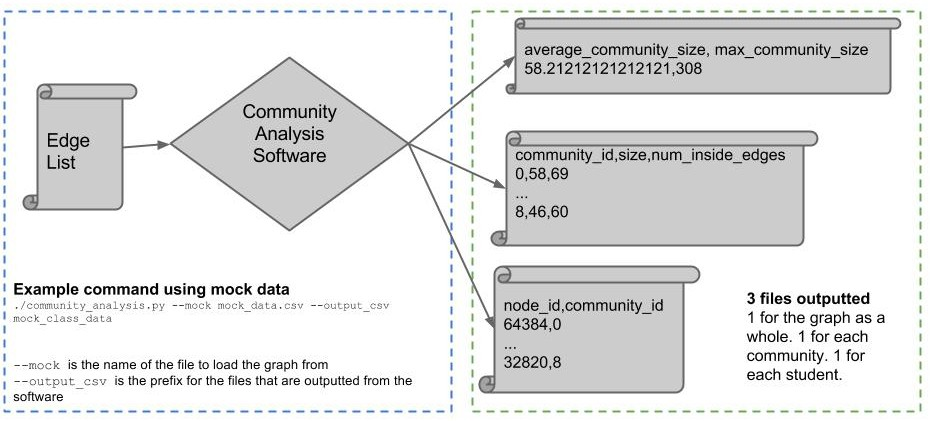
\includegraphics[width=\linewidth]{step2.jpg}
 \caption{CommunityFinder performs analysis on an edge list and output three files that describe the community structure discovered by the graph}
\end{figure}

% \begin{figure}[h]
%  \centering
%  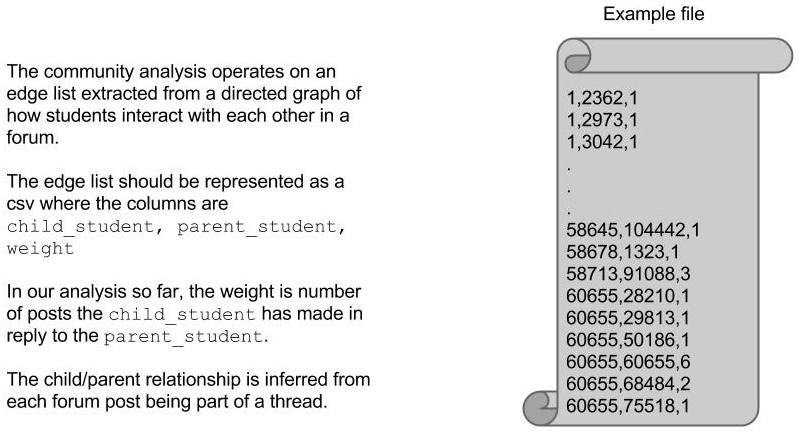
\includegraphics[width=.8\linewidth]{step1.jpg}
%  \caption{The first step in using CommunityFinder is to extract the edge list.}
% \end{figure}


\subsection{Data Sources}
In order to extract an Interaction Graph for analysis, CommunityFinder can query from multiple data sources. Currently, it supports a MySQL database in the MOOCdb \cite{veeramachaneni2013moocdb} format, a Mongo database dump as provied from edX, and an edge list formatted as a file of comma separated values. We recommend using MOOCdb as it is a standardized schema for representing MOOC data.

\subsection{Design Decisions}
CommunityFinder is built with flexibility in mind. It is not meant to be tied to an specific MOOC platform. To this end, it is has support for querying directly from any course data that is in the standardized MOOCDB schema. This is the recommended way to use the software.

\begin{figure}[h]
 \centering
 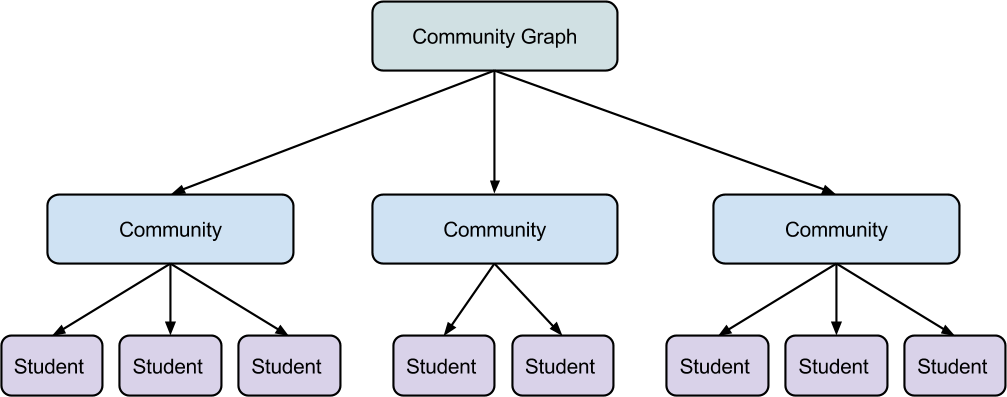
\includegraphics[width=.8\linewidth]{design.png}
 \caption{This represents how the CommnityFinder software understands the structure of the interaction graph. The hierarchical structure was chosen to enable flexibility as the software is developed. }
 \label{design}
\end{figure}

However, it is easy to extend the software to support other data sources. Included in the initial release is support for extracting graph structure from the Mongo database dumps that the edX platform creates. 

Even more, the software supports users who provide their own dataset. An edge list represented as a CSV can be used for analysis by this software. This means that it is possible to use CommunityFinder to find community structure in any graph.

The software organizes the Interaction Graph into a hierarchy of higher level features as shown in Figure \ref{design}. Students are the lowest level. Students are defined by an individual who post on the forum. Student are grouped together to forum communities. A community is a collection of students and has connections to other communities. This hierarchy has a few important implications

\begin{itemize}
\item It is how the data is structured to be exported from the software. This tool is not meant to do analysis beyond community identification. Thus, it is important that the software exports all relevent features about the community structure of the graph that later stages of analysis might use. On the practical side, this structure enabling the programming of additional features for each of the levels. 

\item It gives a good building block for extending functionality. As I discuss the Future Work section, we might want add higher level abstractions such as how the communities develop over time in a class. In order to do this, we simply can create a higher level abstraction that relates several community graph objects.
\end{itemize}

\subsection{Adding Functionality}
Each file that the program outputs is the enumeration of instances of a particular part of the hierarchy in Figure \ref{design}. Right now, these are CommunityGraph, Community, and Student. This means that CommunityFinder outputs a file of comma separated values for each instance at each level. The values that are output depend on the list of properties at the top of each class definition. To add another property, simply add a string to this list. The proprieties can involve additional computation by using python decorators to label certain methods as properties. 


\section{Results}
% \centering
% \begin{tabular}{l*{6}{c}r}
% Method & Number of Communities & Modularity \\
% \hline
% Louvain & 22 & .430\\
% Spectral & 89 & .369\\
% Spectral & 22 & .278\\
% \end{tabular}
% \caption{The performance on optimizing modularity for 6.002x Spring 2012. }
% \label{method}
% \end{table}{}
The Louvain Method has the advantage of not requiring that that number of communities be explicitly set when running the algorithm. For spectral clustering, we simply try all possible values for the number of communities between 1 and the half the total students in the class and present the partition of the highest modularity.

Using CommunityFinder, we extracted the Interaction Graph from two past edX offerings of the course 6.002x. We note that CommunityFinder only counts students that had an interaction with at least 1 other student. The results of running CommunityFinder are presented in Table \ref{results}.

\begin{table}[!htb]
\centering
% \begin{center}
    \begin{tabular}{l*{6}{c}r}
    Course & 6.002x &  6.002x & 6.002x & 6.002x & 6.002x\\
    Offering & Spring 2012 & Fall 2012 & Fall 2012 & Spring 2012 & Spring 2013 \\
    \hline
    Method & Louvain & Louvain & Spectral & Louvain & Spectral \\
    Number of Students & 8816 & 2163 & 2163  & 710 & 710 & \\
    Number of Edges & 52362 & 5641 & 5641 & 1564 & 1564 \\
    Number of Posts & 71440 & 6902 & 6902 & 1914 & 1914 \\
    Number of Communities & 37 & 77 & 114 & 32 & 72 \\
    Average Community Size & 238.3 & 19.0 & 22.1 & 20.3 & 9.9\\
    Largest Community & 1438 & 204 & 413 & 87 & 76 \\
    Modularity & .360 & .510 & .442 & .539 & .502 \\
    \end{tabular}
% \end{center}
\caption{Summary of results of running CommunityFinder 3 edX offerings of 6.002x. We do not present the results of 6.002x Spring 2012 using the spectral clustering because CommunityFinder ran out of memory during the testing for that course.}
\label{results}
\end{table} 


The running time of these community detection algorithms is also an important consideration if we want to be able to analyze a large number of classes. Table \ref{time} shows the running time for 6.002x Fall 2012. 

\begin{table}[!htb]
\centering
% \begin{center}
    \begin{tabular}{l*{6}{c}r}
    Method & Louvain & Spectral 10 communities & Spectral 50 communities & Spectral 100 communities\\
    \hline
    Running Time & .792 sec & 3.300 sec  & 5.068 sec & 6.630 sec \\
    \end{tabular}
% \end{center} 
\caption{The total running times for CommunityFinder under different parameters.}
\label{time}
\end{table} 

\begin{figure}[!htb]
  \centering
  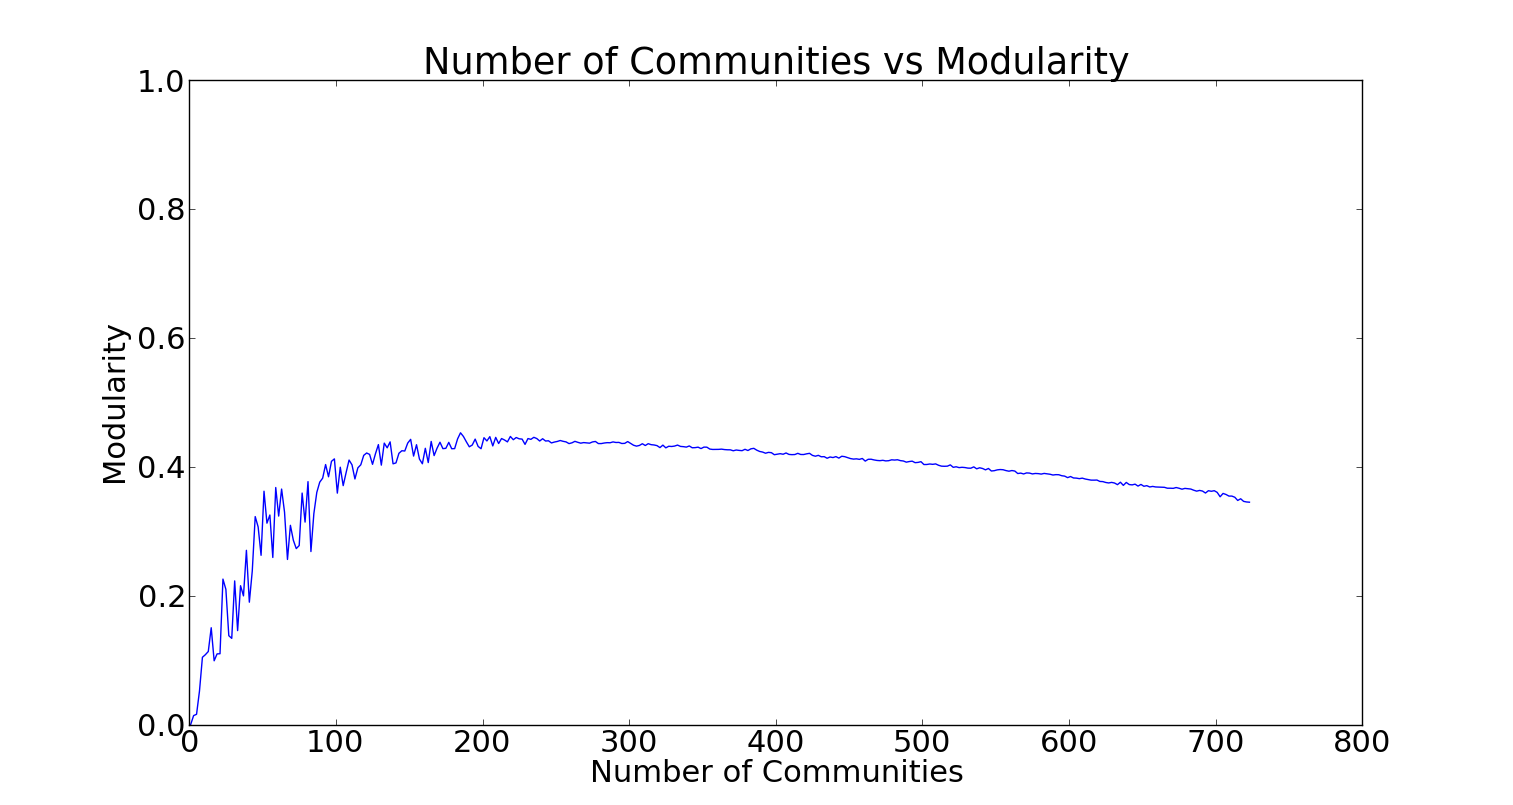
\includegraphics[width=.8\linewidth]{modularityf12.png}
  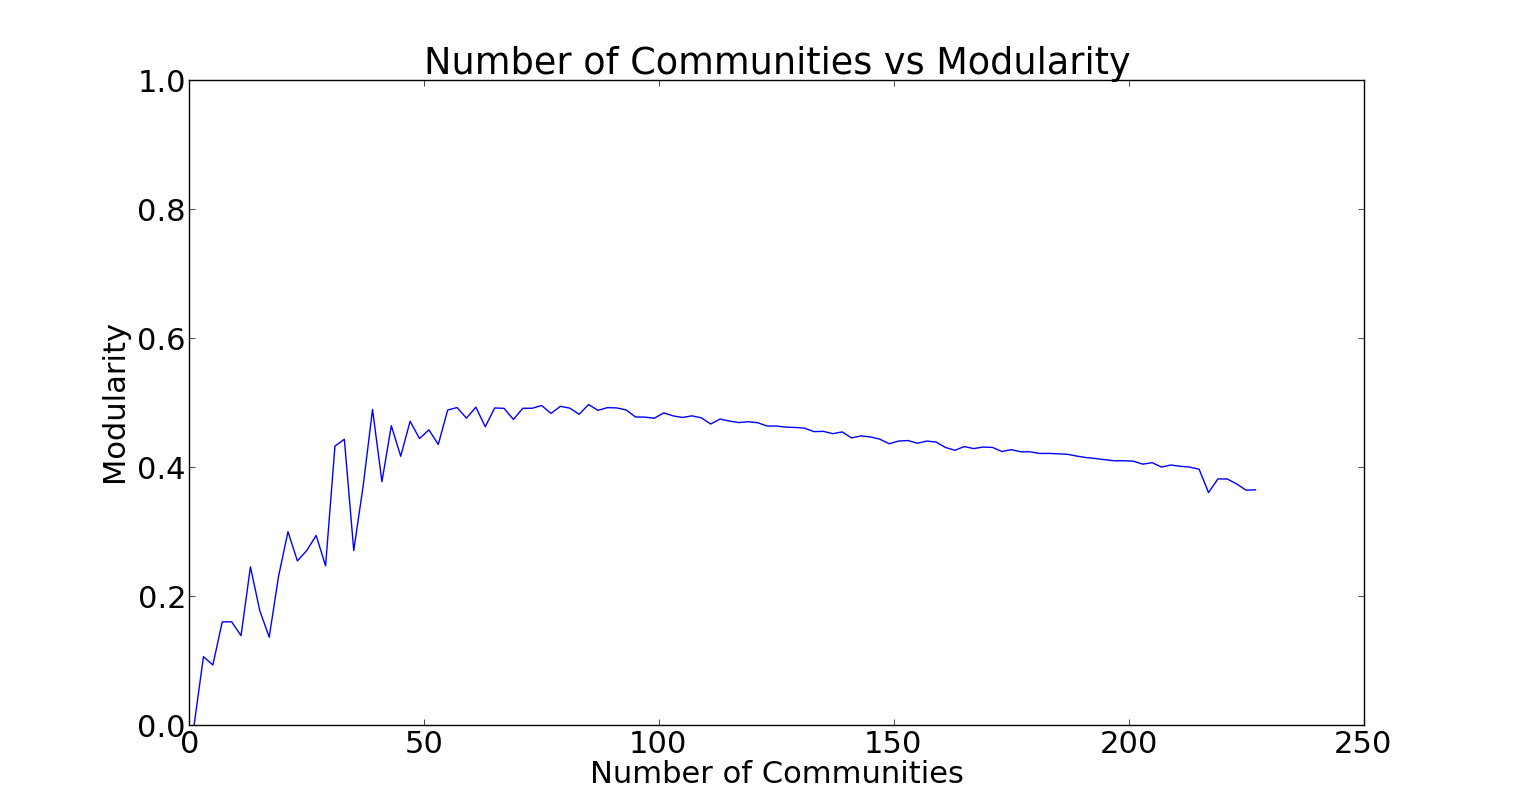
\includegraphics[width=.8\linewidth]{modularitys13.png}
  \caption{Number of Communities vs Modularity. 6.002x Fall 2012 is on top and 6.002x Spring 2013 is on bottom}
  \label{modularity}
\end{figure}



Unlike Louvain Method, spectral clustering requires the number of communities in order to produce a result. The result we present in Table \ref{results} show the number of clusters that achieves the highest modularity. Figure \ref{modularity} shows how the number of communities specified affects the modularity of interaction graph for 6.002x Fall 2012. 



% \begin{figure}[!htb]
%     \centering
%     \caption{Best Spectral Partition for 6.002x Spring 2012}
%     \label{spectral_best}
% \end{figure}

% \begin{figure}[!htb]
%     \centering
%     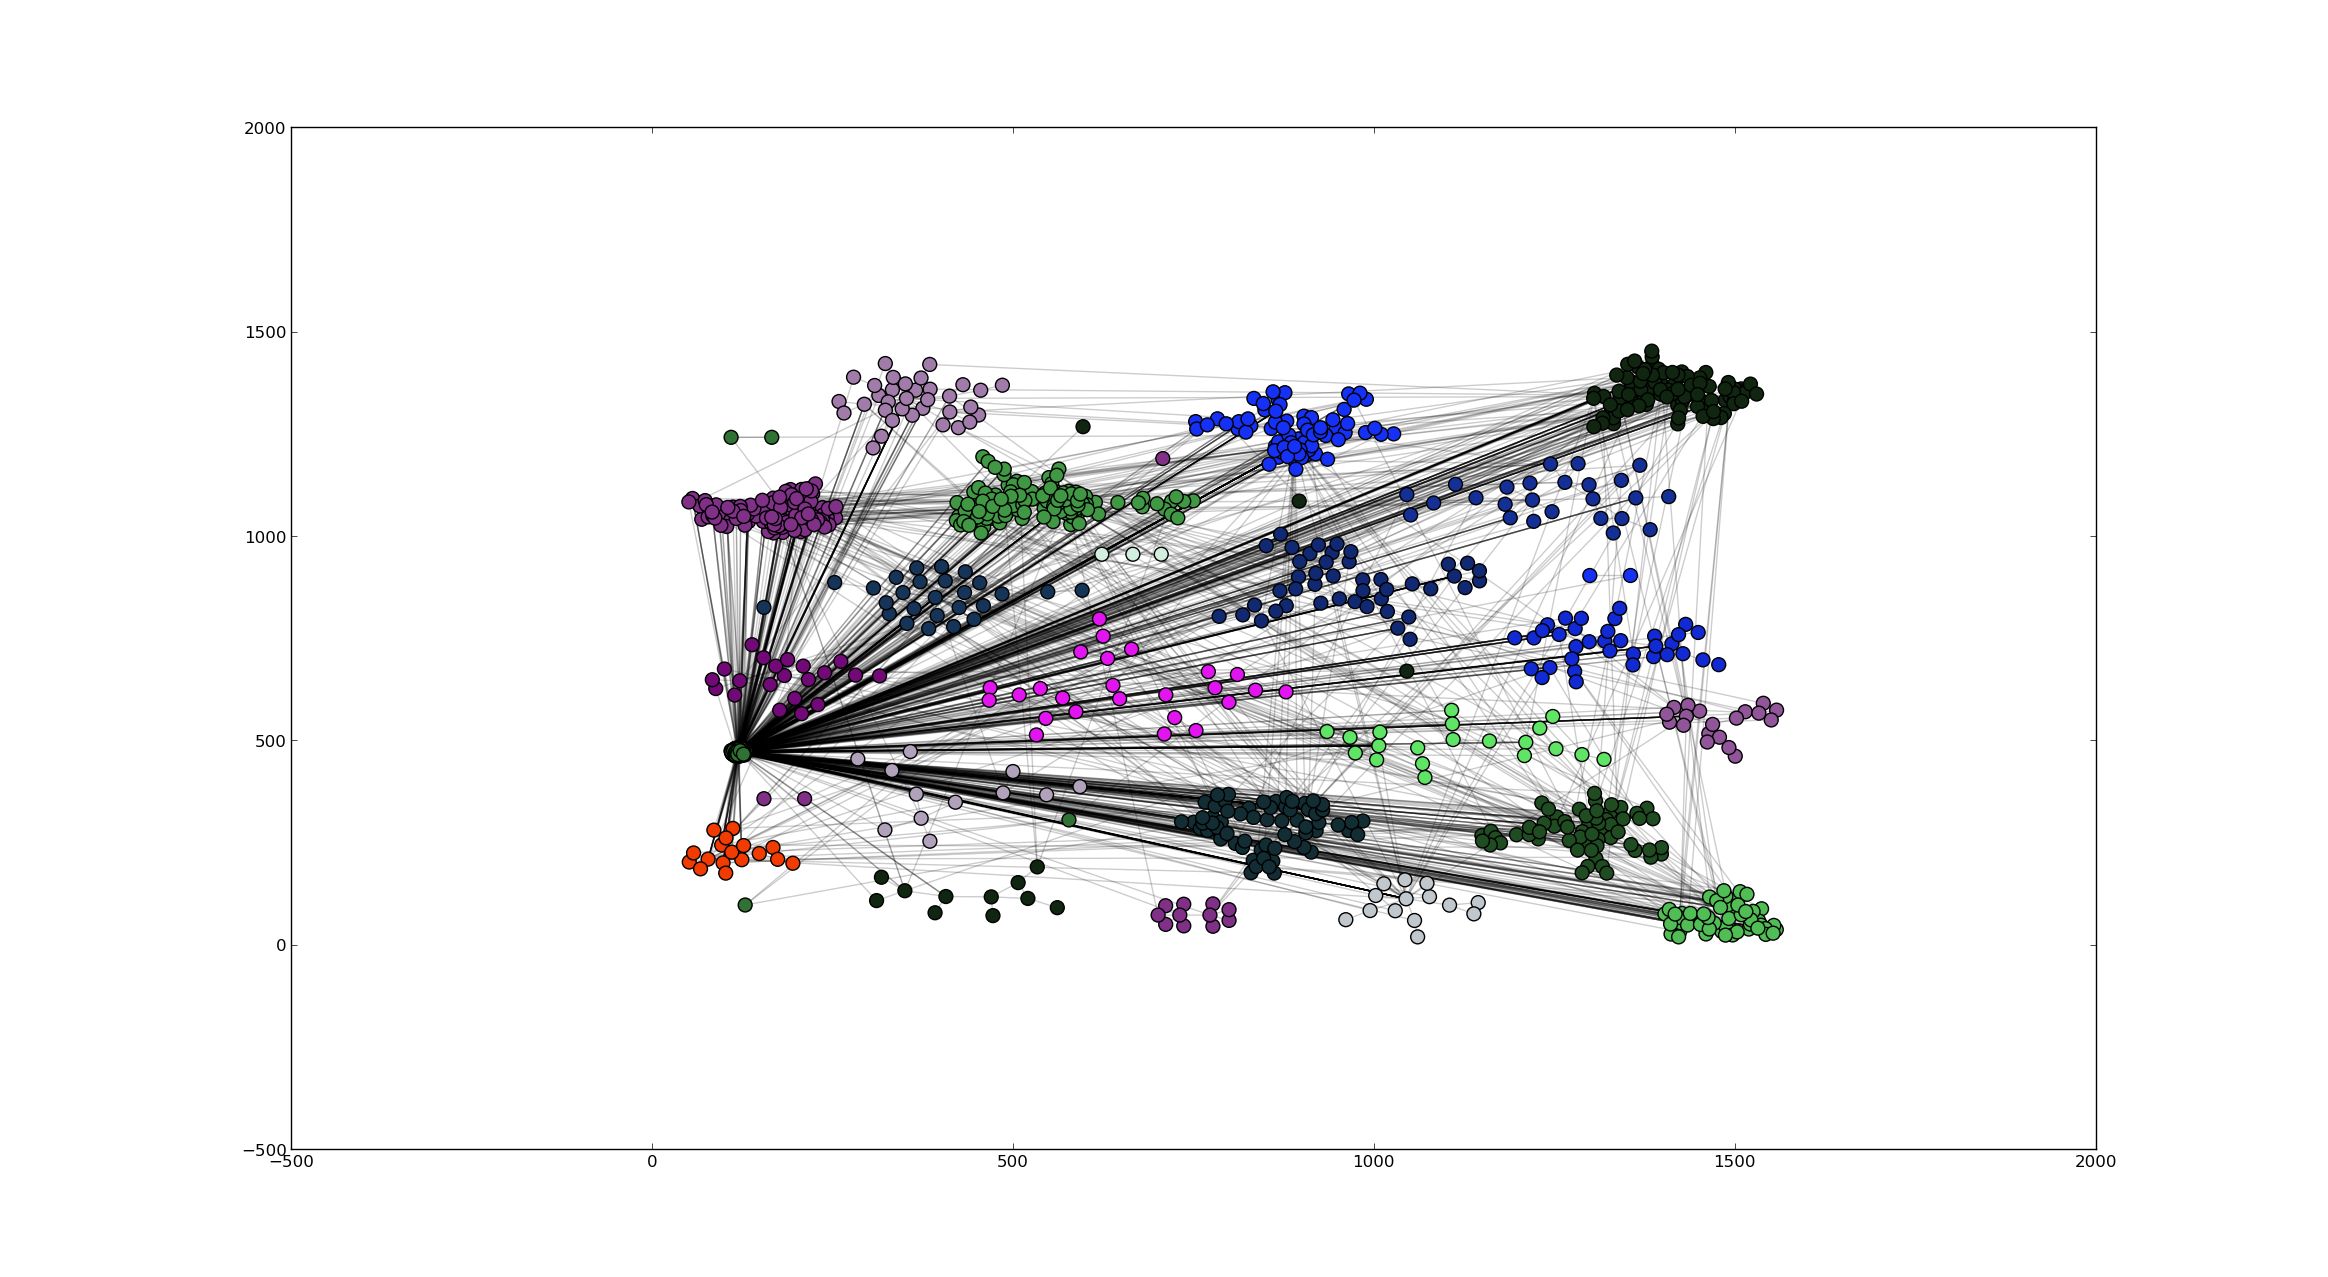
\includegraphics[width=.8\linewidth]{spectral_22.png}
%     \caption{Spectral Partition with 22 communities for 6.002x Spring 2012}
%     \label{spectral_22}
% \end{figure}






\section{Discussion}
The initial results show the Louvain Method obtains a higher modularity than spectral clustering in two offerings of 6.002x. In the third offering, only the Louvain Method produced results. The Louvain Method also achieves this maximum modularity with a lower number of of communities when compared to spectral clustering.

Spectral clustering requires the number of communities to be specified. In order to optimize modularity, CommunityFinder does a brute force search over the number of communities. Figure \ref{modularity} shows how the modularity varies as we vary the number of communities. We can see that increasing the number of communities increase modularity up to a certain point. After that, further increases in number of communities decreases the modularity. 

The other important consideration is performance. The Louvain Method vary clearly outperforms spectral clustering on our dataset. The running time of Louvain method for 6.002x Fall 2012 is nearly 10x faster than using spectral clustering to determine 100 communities on equivalent Interaction Graph. The advantage becomes clearer when we determine the optimal number of communities in spectral clustering because we must actually run the the algorithm multiple times. For example, in our testing, we tested nearly 700 different values for the number of communities in 6.002x Fall 2012. This further amplifies the performance advantage of the Louvain Method.

Overall, these two results suggest that the Louvian Method is better for community detection under the goal of modularity optimization. If we consider another metric the results may change. Additionally, we only ran this analysis on three datasets, all from offerings the same course. We may see different results for other courses, especially ones in disciplines other than computer science.

\section{Contributions}


\begin{itemize}
  \item Described how to transform a corpus of forum posts into an Interaction Graph
  \item Examined 2 methods for community detection on an Interaction Graph and presented intital results
  \item Implemented software to extract Interaction Graph from various representation of the raw data and run community analysis.
%   \item Published  anonymoized datasets from 6.002x Fall 2012 and Spring 2013 
\end{itemize}

\section{Future Work}

CommunityFinder is first and foremost a tool to do community analysis. As such, it is meant to be used to do further research on MOOCs. The functionality should grow to accommodate the needs of the people using the tool. Thus, it will be important to see how people use CommunityFinder.

The are a few good ideas already for future features. For instance, CommunityFinder could implement other community detection algorithms. There has been a lot of work on other algorithm that have not been tested. Some of the most interesting are the ones that do not limit a student to being in only one community. Developing support overlapping communities is a one possible future feature. A second feature is one that tracks how community structure changes over time. Researchers might want to know how a community morphs week to week in order to assess how effectively course material is being taught.

Finally, an interesting project would be to use CommunityFinder to relate superposters (as identified by Huang et al.) to their community assignment.









\bibliographystyle{plain}
\bibliography{bibliography}
%\include{bibliography.tex}

\newpage
\newappendix{Base Class for Data Source}
\lstinputlisting[language=Python, showstringspaces=false]{code0.py}
\newpage

\newappendix{Class for Mock Data Source }
\lstinputlisting[language=Python, showstringspaces=false]{code1.py}
\newpage

\newappendix{Class for MOOCdb Data Source }
\lstinputlisting[language=Python, showstringspaces=false]{code2.py}
\newpage

\newappendix{Class for MongoDB Data Source }
\lstinputlisting[language=Python, showstringspaces=false]{code3.py}
\newpage







\end{document}

%-------------------------------------------------------------------------




